\documentclass[12pt,a4paper]{extarticle}
\usepackage[margin=2cm]{geometry}
\usepackage[slantfont,boldfont]{xeCJK}
\usepackage{graphicx}
\usepackage{caption}
\usepackage{float}
\usepackage{amssymb}
\usepackage{amsmath}
\usepackage{pgfplots}
\usepackage{subcaption}

\graphicspath{{./images/}}
\pgfplotsset{compat=1.12}
\setCJKmainfont{cwTeXKai}

\title{Machine Learning 2017 Spring\\Homework 4 Report}
\author{學號:\texttt{B03902048}\\系級:資工三\\姓名:林義聖}
\date{}

\begin{document}
\maketitle

\begin{itemize}

  \item[1.1] Dataset 中前 10 個人的前 10 張照片的平均臉和 PCA 得到的前 9 個 eigenfaces。
  \par 答:平均臉呈現在 Figure \ref{fig:average-face},而 eigenfaces 在 Figure \ref{fig:top-9-eigenfaces}。

  \begin{figure}[ht]
    \begin{subfigure}[t]{0.5\textwidth}
      \centering
      
\includegraphics[width=0.8\linewidth]{average-face.png}
      \caption{The average face}
      \label{fig:average-face}
    \end{subfigure}
    \begin{subfigure}[t]{0.5\textwidth}
      \centering
      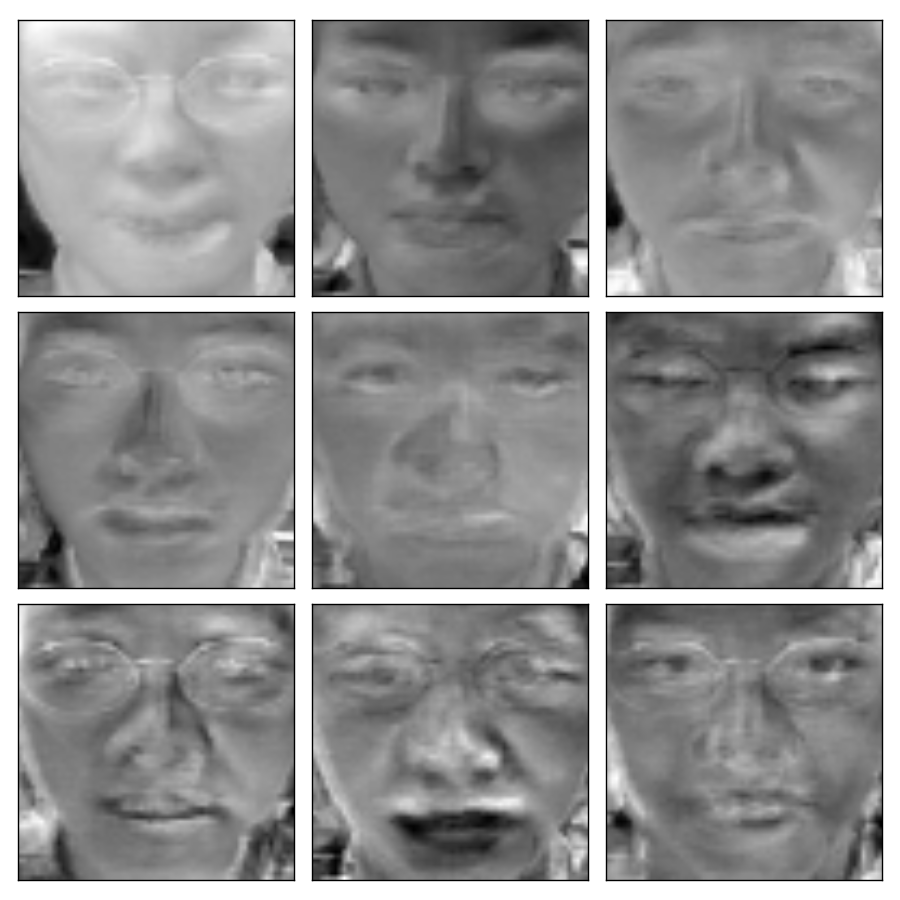
\includegraphics[width=0.8\linewidth]{eigen-faces-top-9.png}
      \caption{The top 9 eigenfaces}
      \label{fig:top-9-eigenfaces}
    \end{subfigure}
    \caption{}
  \end{figure}

  \item[1.2] Dataset 中前 10 個人的前 10 張照片的原始圖片和 reconstruct 圖(用前 5 個 eigenfaces)。
  \par 答:Figure \ref{fig:original-faces} 是原始圖片,而 Figure \ref{fig:recovered-faces} 是使用 eigenfaces 重建的圖片。

  \begin{figure}[ht]
    \begin{subfigure}[t]{0.5\textwidth}
      \centering
      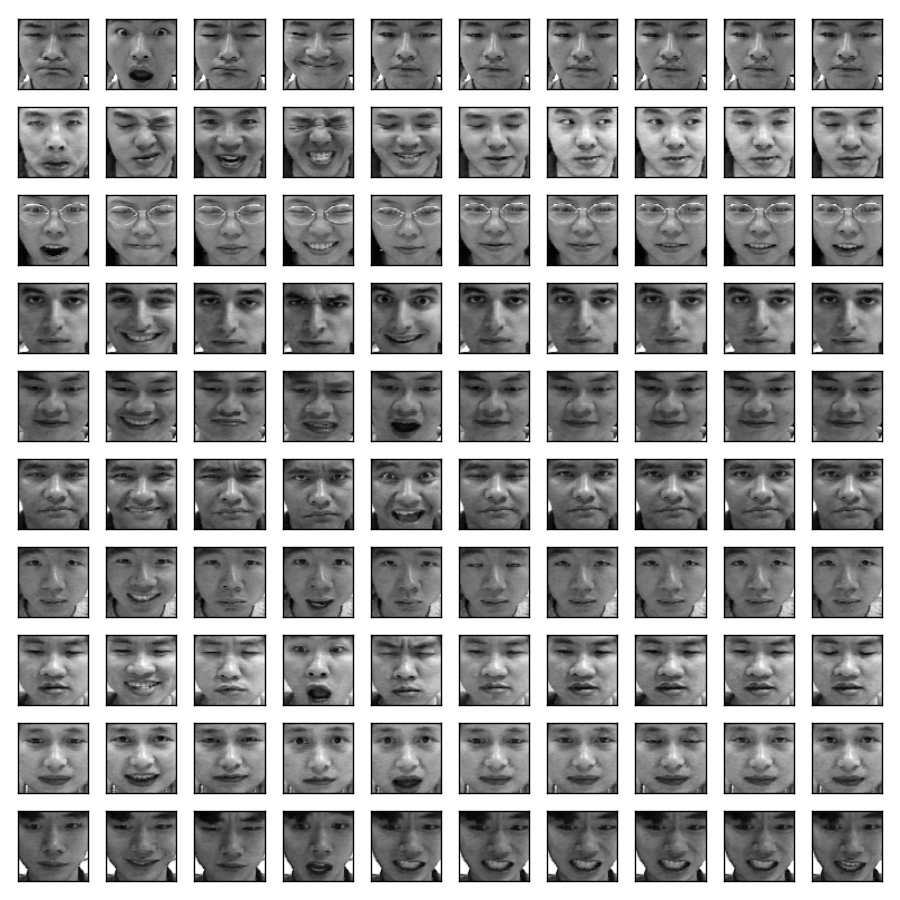
\includegraphics[width=\linewidth]{origin-faces-first-100.png}
      \caption{Original faces}
      \label{fig:original-faces}
    \end{subfigure}
    \begin{subfigure}[t]{0.5\textwidth}
      \centering
      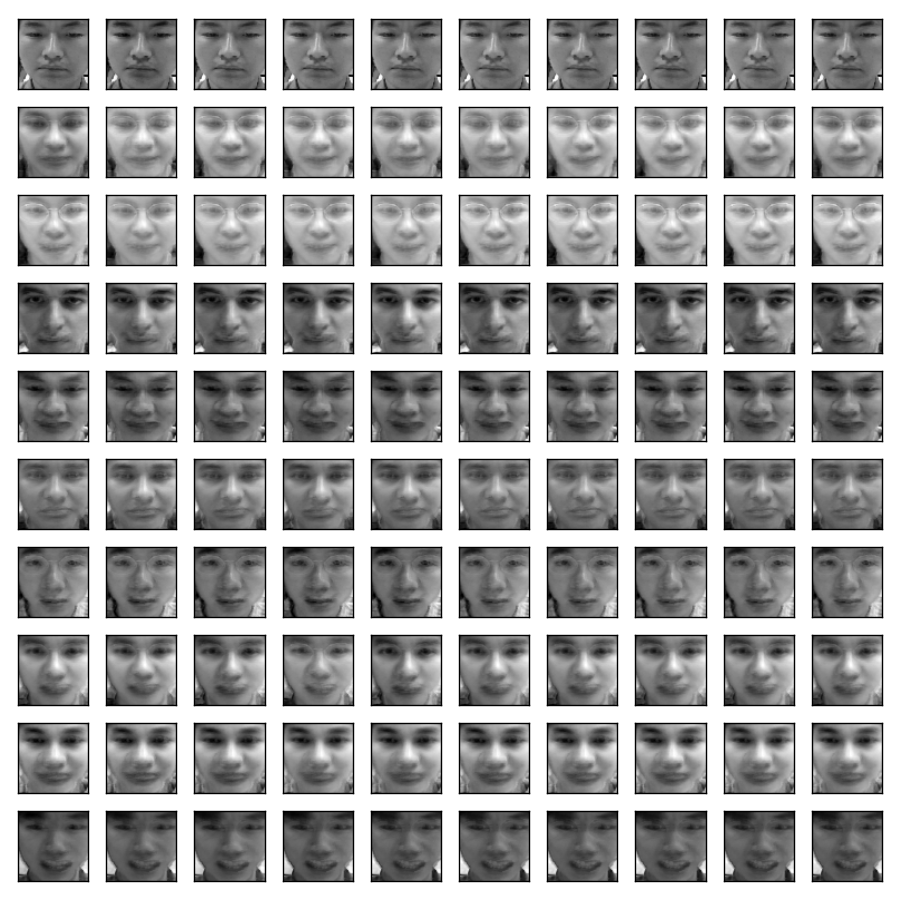
\includegraphics[width=\linewidth]{reconstruct-with-5-eigenfaces.png}
      \caption{Recovered faces}
      \label{fig:recovered-faces}
    \end{subfigure}
    \caption{100 faces reconstructed with top 5 eigenfaces}
    \label{fig:reconstruct-with-eigenfaces}
  \end{figure}

  \item[1.3] Dataset 中前 10 個人的前 10 張照片投影到 top $k$ eigenfaces 時就可以達到 < 1\% 的 reconstruction error?
  \par 答:當 $k = 59$ 時可以達到。

  \item[2.1] 使用 word2vec toolkit 的各個參數的值與其意義。
  \par 答:我訓練 word2vec 模型時,使用的是 default 參數,並將 vector size 設為 64。
  \begin{itemize}
    \item word2phrase
    \par 有時原始的 data 中會有許多固定擺在一起的單字,如:地點、特殊名詞等,使用 word2phrase 可以將這樣的字組合起來視作一個單字。
    \item word2vec
    \begin{itemize}
      \item size:指定 vector size,將所有 word 以這個大小的 vector 表示。
      \item window:指定 skip-grams 的 window 大小。因為在做 skip-grams 的時候,給定一個「詞窗」罩住 $w$ 這個單字而形成一個句子,而 skip-grams 就是在預測詞窗中缺漏的字 $c$,而給出機率 $p(c|w)$。因而 window 大小,就決定了模型最多會跨過多少單詞距離,給出機率 $p(c|w)$。
      \item sample:在訓練時,大於某個 frequency 的單字有機會被略過,即 downsample。此舉在訓練模型時,可以加速訓練過程。在某些情形下,也能增加準確率。
      \item hs:指定是否使用 Hierarchical Softmax。因為原先情況下,單純使用 softmax,輸出時要計算的參數數量很龐大。而透過訓練前先把單詞分類,建立階層式的輸出,就可以一層一層地判斷類別,大幅減少計算量。
      \item min\_count:指定是否忽略 frequency 小於這個數值的字。
      \item alpha:即 learning rate 初始值。
      \item cbow:預設是使用 skip-grams,可以改為使用 CBOW。相對於 skip-grams 是給定 $w$ 預測 $c$,CBOW 則是給定 $c$ 預測當前的字 $w$,即給出 $p(w|c)$。
    \end{itemize}
  \end{itemize}

  \item[2.2] 將 word2vec 的結果投影到 2 維的圖。
  \par 答:我選擇頻率最高的 1000 個字,挑選過後剩下 381 個,呈現在 Figure \ref{fig:wordvec-es64-top1000}。

  \begin{figure}[ht]
    \centering
    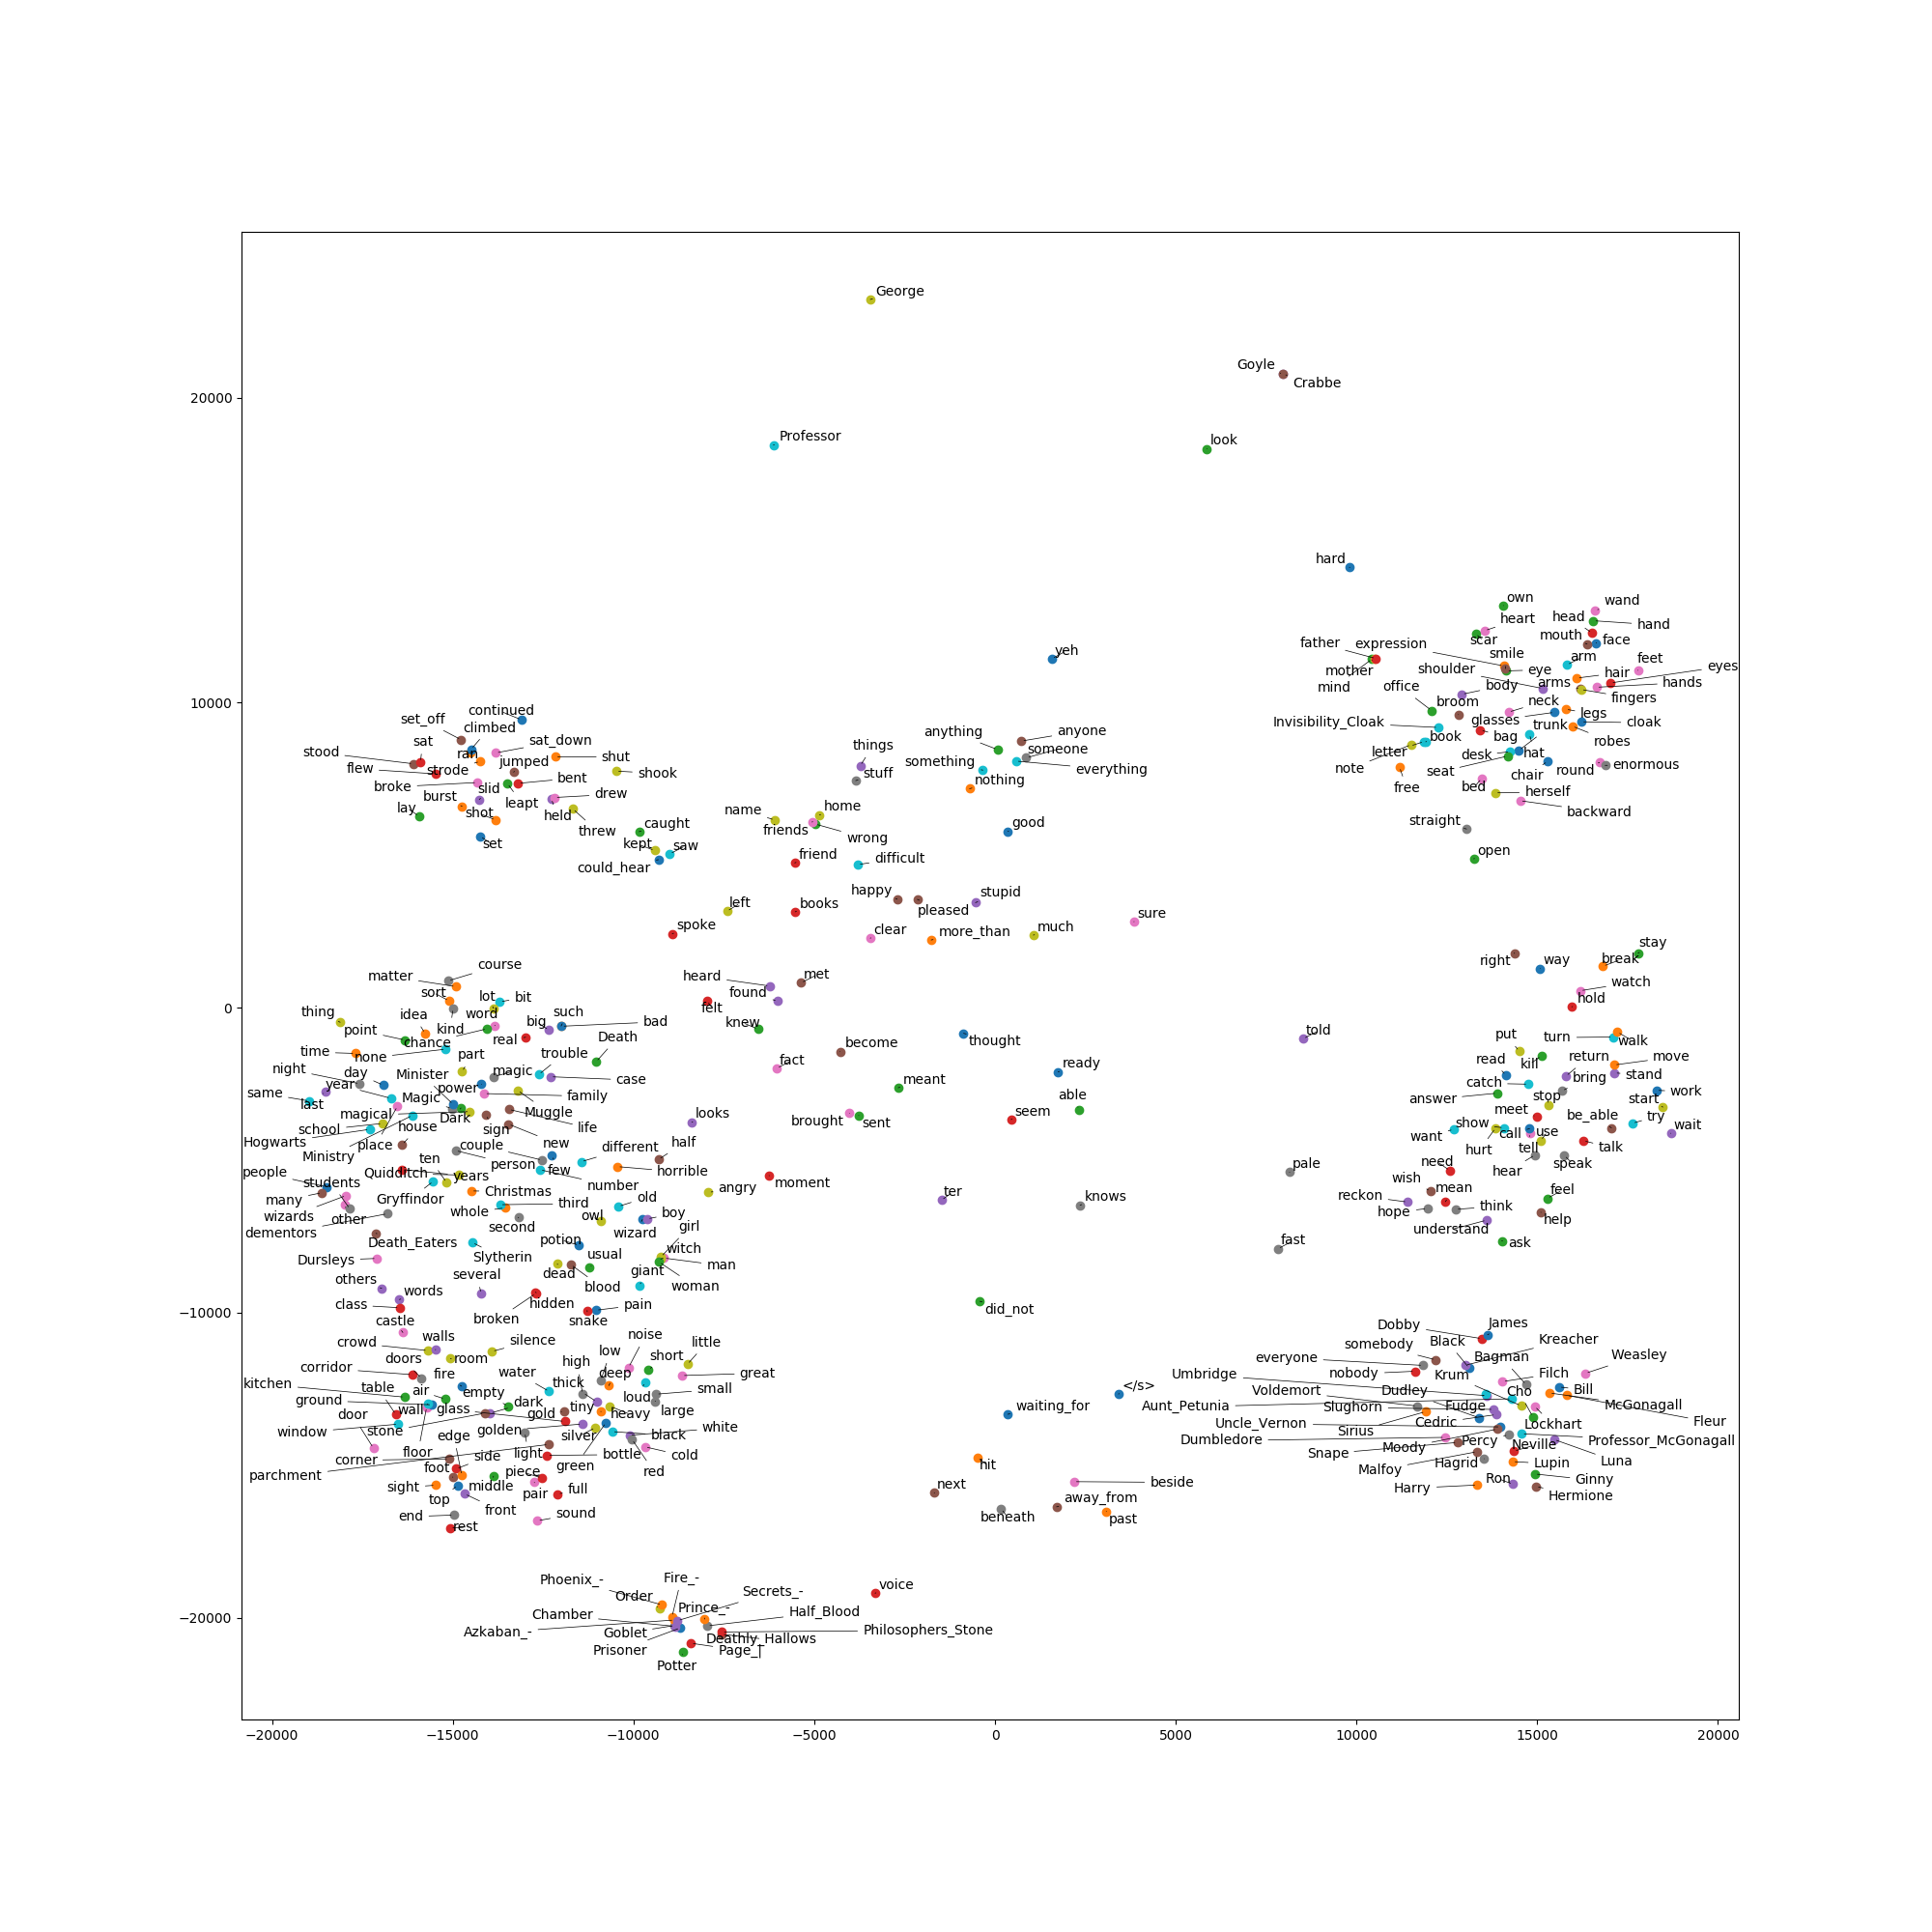
\includegraphics[width=0.8\linewidth]{images/wordvec-es64-top1000.png}
    \caption{The top 1000 frequent words}
    \label{fig:wordvec-es64-top1000}
  \end{figure}

  \item[2.3] 從上題視覺化的圖中觀察到了什麼?
  \par 答:從 Figure \ref{fig:wordvec-es64-top1000} 中,我觀察到「人名」聚集在圖片右下方,圖片右方中間則是一些「原型動詞」,右上方則比較特別,聚集了「身體部位」和「家具」。圖片最下方是「書名」,推測是因為訓練資料中每個頁面下方都會有書名,所以它們出現的頻率很高。圖片左下方是一堆「形容詞」,而鄰近它們的上方是一些「名詞」,圖片的左方偏上則是「過去式動詞」。

  \item[3.1] 請詳加解釋你估計原始維度的原理、合理性,這方法的通用性如何?
  \par 答:
  \begin{enumerate}
    \item 我利用 \texttt{gen.py} 多次生成 10000 筆 sample data,其中 $d_i \in [1, 60], h_i \in [60, 79]$,所以共有 1200 組 sample data,稱之為 $X_i, i = 1, 2, \dots, 1200$
    \item 計算 $X_i$ 的標準差 $\hat{\sigma}_{X_i}$。通過觀察,我發現隨著 $d_i$ 增大,$\hat{\sigma}_{X_i}$ 也會隨之增加
    \item 計算測資 $S_i, i = 1, 2, \dots, 200$ 的標準差 $\hat{\sigma}_{S_i}$
    \item 將 $\hat{\sigma}_{S_i}$ 與 $d_i$ 相同但 $h_i$ 不同的 20 個 $\hat{\sigma}_{X_i}$ 相減,並取其平均值 $\mu_{d_i}$
    \item 對於每個 $S_i$,另 $\tilde{d_i} = \underset{d_i}{\arg\min}\ \mu_{d_i}$
  \end{enumerate}
  \par 這個作法的原理及合理性,其實就是利用統計方法,觀察隨著 $d_i$ 不同時,產生出來的資料在統計上有什麼特性。透過簡單的觀察,我發現整組 sample data 的標準差會隨著 $d_i$ 增加而上升。然而,這個方法是鐵定不通用的。舉例來說:對於任意要預測 $\tilde{d_i}$ 的一組測資,若是他經過標準化後,標準差隨即變成 1,這時再用我這個方法就完全不可靠了。

  \item[3.2] 將你的方法做在 hand rotation sequence datatset 上得到什麼結果?合理嗎?請討論之。
  \par 答:透過上述方法,我先將 481 張照片讀進來並攤平,將他們視做 481 個點,並計算這些點的標準差後,預測出這組 dataset 的 $\tilde{d_i} = 31$。顯然這是不合理的,因為這些資料並不是由 normal distribution 生成,再透過 neural network 轉換到高維度的,必然會有很不同的統計性質。根據推測,這組 dataset 的 $\tilde{d_i}$ 應該很接近 3,因為這些照片所呈現的,是一個三維度空間中的資訊。

\end{itemize}

\end{document}
